\documentclass[../../main.tex]{subfiles}
\begin{document}

{\bf [解答]}

\paragraph{(1)}

与えられた方程式
\begin{align}
  x(x-3)(x+3)+3k(x-1)(x+1)=0 \quad (k>0) \label{eq:1}
\end{align}
について考える．$x = \pm 1$ は解でないから両辺$(x-1)(x+1)$で割って
\begin{align}
  k = \dfrac{-x(x-3)(x+3)}{3(x+1)(x-1)} = \dfrac{1}{3}\left[ -x + \dfrac{8x}{x^2-1} \right] \equiv f(x) \label{eq:2}
\end{align}
である．ここで
\begin{align}
  f(x) = \dfrac{1}{3}\left[-x + \dfrac{8x}{x^2-1}\right] \label{eq:3}
\end{align}
とおいた．一階微分は
\begin{align}
  3f'(x)
  & = -1 + \dfrac{8(x^2-1) - 8x \cdot 2x}{(x^2-1)^2} \\
  & = -1 + \dfrac{-8x^2-8}{(x^2-1)^2} \\
  & = \dfrac{-(x^2+3)^2}{(x^2-1)^2} < 0
\end{align}
となって$f'(x)<0$つまり $f(x)$ は $x < -1, -1 < x < 1, 1 < x$ の各区間で単調減少である．不連続点と無限遠での極限値は
\begin{align}
  \begin{cases}
    f(x) &\longrightarrow \mp \infty \quad (x \to \pm \infty) \\
    f(x) &\longrightarrow \pm \infty \quad (x \to -1 \pm 0) \qquad (\text{複号同順}) \\
    f(x) &\longrightarrow \pm \infty \quad (x \to 1 \pm 0)
  \end{cases}
\end{align}
だから，$y=f(x)$の増減表とグラフは下図のようになる．
\cref{eq:1}の解は$y=f(x)$と$y=k$の交点に対応するから，いかなる$k (>0)$に対しても交点すなわち解は$3$つある．よって題意は示された．

\begin{table}[htb]
  \centering
  \caption{$f(x)$ の増減表}
  \label{tab:1967_1_variation}
  \begin{tabular}{c|ccccc}
    $x$ & $\cdots$ & $-1$ & $\cdots$ & $1$ & $\cdots$ \\ \hline
    $f'(x)$ & $-$ & & $-$ & & $-$ \\ \hline
    $f(x)$ & $\searrow$ & & $\searrow$ & & $\searrow$
  \end{tabular}
\end{table}

\begin{figure}[htb]
  \centering
  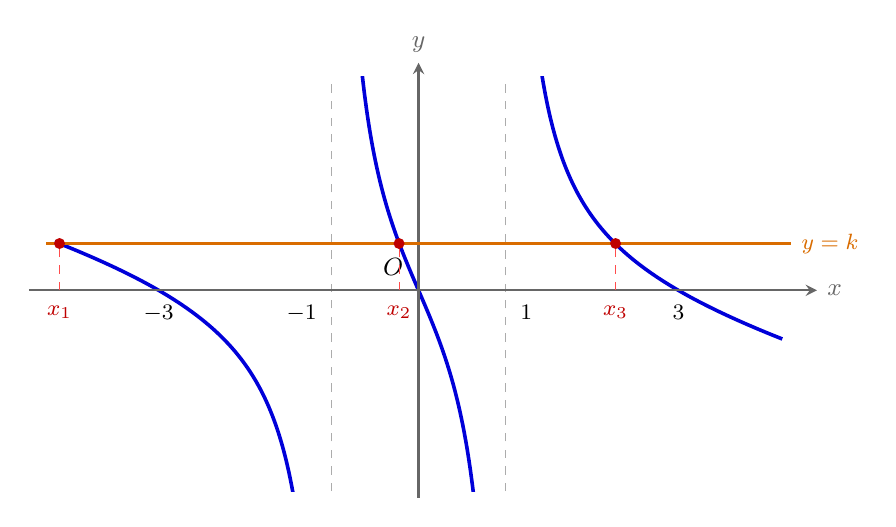
\begin{tikzpicture}[x=1.1cm, y=0.85cm, >=stealth,
    every node/.style={font=\small}]
    % 漸近線
    \draw[dashed, gray!65] (-1, -3.0) -- (-1, 3.2);
    \draw[dashed, gray!65] (1, -3.0) -- (1, 3.2);

    % 曲線 y = f(x)
    \begin{scope}
      \clip (-4.3, -3.0) rectangle (4.3, 3.2);
      \draw[line width=1.3pt, blue!85!black, domain=-4.2:-1.06, samples=160, smooth]
      plot (\x, {-\x*(\x-3)*(\x+3)/(3*(\x+1)*(\x-1))});
      \draw[line width=1.3pt, blue!85!black, domain=-0.94:0.94, samples=160, smooth]
      plot (\x, {-\x*(\x-3)*(\x+3)/(3*(\x+1)*(\x-1))});
      \draw[line width=1.3pt, blue!85!black, domain=1.06:4.2, samples=160, smooth]
      plot (\x, {-\x*(\x-3)*(\x+3)/(3*(\x+1)*(\x-1))});
    \end{scope}

    % 座標軸
    \draw[->, thick, gray!80!black] (-4.5, 0) -- (4.6, 0) node[right] {$x$};
    \draw[->, thick, gray!80!black] (0, -3.1) -- (0, 3.4) node[above] {$y$};
    \node[above left=2pt] at (0, 0) {$O$};

    % 直線 y = k
    \draw[line width=1.1pt, orange!85!black] (-4.3, 0.7) -- (4.3, 0.7)
    node[right, font=\footnotesize] {$y = k$};

    % 交点 3つ (k=0.7)
    \coordinate (P1) at (-4.145, 0.7);
    \coordinate (P2) at (-0.225, 0.7);
    \coordinate (P3) at (2.275, 0.7);

    \draw[dashed, red!70] (-4.145, 0) -- (P1);
    \draw[dashed, red!70] (-0.225, 0) -- (P2);
    \draw[dashed, red!70] (2.275, 0) -- (P3);

    \node[circle, fill=red!75!black, inner sep=1.4pt] at (P1) {};
    \node[circle, fill=red!75!black, inner sep=1.4pt] at (P2) {};
    \node[circle, fill=red!75!black, inner sep=1.4pt] at (P3) {};

    \node[below=2pt, font=\footnotesize] at (-3, 0) {$-3$};
    \node[below left=2pt, font=\footnotesize] at (-1, 0) {$-1$};
    \node[below right=2pt, font=\footnotesize] at (1, 0) {$1$};
    \node[below=2pt, font=\footnotesize] at (3, 0) {$3$};

    \node[below=2pt, red!75!black, font=\footnotesize] at (-4.145, 0) {$x_1$};
    \node[below=2pt, red!75!black, font=\footnotesize] at (-0.225, 0) {$x_2$};
    \node[below=2pt, red!75!black, font=\footnotesize] at (2.275, 0) {$x_3$};
  \end{tikzpicture}
  \caption{$y = f(x)$ と直線 $y = k$ の交点（実根が3個存在する様子）}
  \label{fig:1967_1_three_roots}
\end{figure}

\paragraph{(2)}

\begin{figure}[htb]
  \centering
  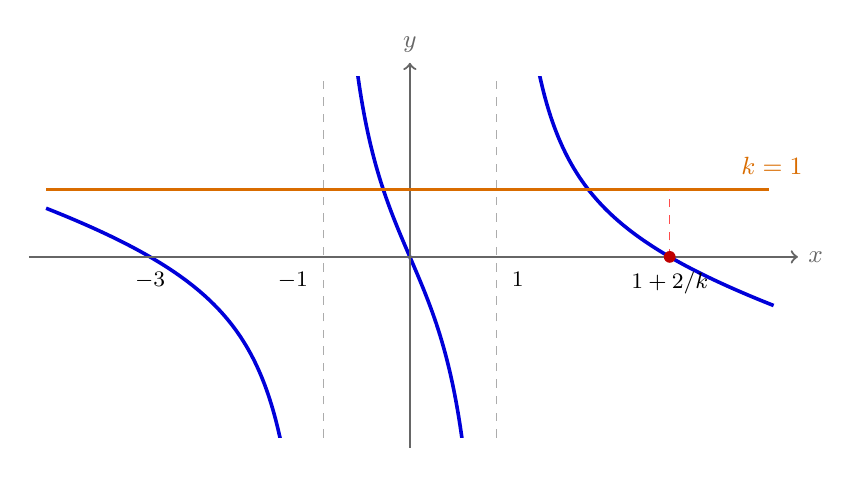
\begin{tikzpicture}[x=1.1cm, y=0.85cm,
    every node/.style={font=\small}]
    % Plot k=-x(x-3)(x+3)/(3(x^2-1)); k=1 illustrates part (2).
    \draw[dashed, gray!65] (-1,-2.7)--(-1,2.7)
    (1,-2.7)--(1,2.7);
    \begin{scope}
      \clip (-4.25,-2.7) rectangle (4.25,2.7);
      \draw[line width=1.3pt, blue!85!black,
      domain=-4.2:-1.06, samples=160, smooth]
      plot (\x,{-\x*(\x-3)*(\x+3)/(3*(\x+1)*(\x-1))});
      \draw[line width=1.3pt, blue!85!black,
      domain=-0.94:0.94, samples=160, smooth]
      plot (\x,{-\x*(\x-3)*(\x+3)/(3*(\x+1)*(\x-1))});
      \draw[line width=1.3pt, blue!85!black,
      domain=1.06:4.2, samples=160, smooth]
      plot (\x,{-\x*(\x-3)*(\x+3)/(3*(\x+1)*(\x-1))});
    \end{scope}
    \draw[->, thick, gray!80!black] (-4.4,0)--(4.48,0)
    node[right] {$x$};
    \draw[->, thick, gray!80!black] (0,-2.85)--(0,2.9)
    node[above] {$y$};
    \draw[line width=1.1pt, orange!85!black]
    (-4.2,1)--(4.15,1);
    \node[orange!85!black, above right=2pt] at (3.65,1)
    {$k=1$};
    \draw[dashed, red!70] (3,0)--(3,1);
    \node[circle, fill=red!75!black, inner sep=1.5pt] at (3,0) {};
    \node[below=2pt, font=\footnotesize] at (-3,0) {$-3$};
    \node[below left=2pt, font=\footnotesize] at (-1,0) {$-1$};
    \node[below right=2pt, font=\footnotesize] at (1,0) {$1$};
    \node[below=2pt, font=\footnotesize] at (3,0)
    {$1+2/k$};
  \end{tikzpicture}
  \caption{$k=-x(x-3)(x+3)/(3(x^2-1))$ のグラフ}
  \label{fig:1967_1_roots}
\end{figure}

(1)のグラフより，$k=f(x)$の正の解は$1<x$に限られる．
また，$(1,1+2/k]$の区間では$y=\dfrac{1}{3}f(x)$は単調減少である．
具体的に$x=1+\dfrac{2}{k}$での値を評価すると\cref{eq:3}より
\begin{align}
  3f\left(1+\dfrac{2}{k}\right)
  & = -\left(1+\dfrac{2}{k}\right) + \dfrac{8(1+2/k)}{(1+2/k+1)(1+2/k-1)} \\
  & = -\dfrac{k+2}{k} + \dfrac{8k(k+2)}{2(2+2k)} \\
  & = -\dfrac{k+2}{k} + \dfrac{2k(k+2)}{k+1} \\
  & = \dfrac{-(k+2)(k+1)+2k(k+2)k}{k(k+1)} \\
  & = \dfrac{-(k+2)(-k-1+2k^2)}{k(k+1)} \\
  & = \dfrac{-(k+2)(2k+1)(k-1)}{k(k+1)} \\
  \therefore
  f\left(1+\dfrac{2}{k}\right)
  & = \dfrac{-(k+2)(2k+1)(k-1)}{3k(k+1)}
\end{align}
だから，$k$との大きさを比較すると
\begin{align}
  k - f\left(1+\dfrac{2}{k}\right)
  & = k - \dfrac{(k-1)(k+2)(2k+1)}{3k(k+1)} \\
  & = \dfrac{k^3+3k+2}{3k(k+1)} > 0 \quad (\because k > 0)
\end{align}
より，$k > f\left(1+\dfrac{2}{k}\right)$ となる．一方で
\begin{align}
  \lim_{x\to 1+0} k-f(x) = -\infty
\end{align}
だから，$x\to 1$では$f(x)>k$, $x=1+2/k$では$f(x)<k$となり，$f(x)$の単調性と合わせてこの区間
\begin{align}
  1 < x < 1 + \dfrac{2}{k}
\end{align}
にただ一つの正の解を持つ．

\newpage

\end{document}
